\documentclass[addpoints]{exam}

\usepackage[english]{babel}
\usepackage[utf8x]{inputenc}
\usepackage{listings}
\usepackage{amsmath}
\usepackage{amsfonts}
\usepackage{mathtools}
\usepackage{tikz}
\usepackage{qtree}
\usepackage{tikz-qtree}
\usepackage{graphicx}
\usepackage{enumitem}
\usepackage[norelsize,noline,noend,linesnumbered]{algorithm2e}
\usetikzlibrary{arrows,automata}
\usepackage{hyperref}
\hypersetup{
    colorlinks=true,
    linkcolor=blue,
    filecolor=magenta,
    urlcolor=cyan,
}
\usepackage{mdframed}


\begin{document}

\title{CS260 - Written Assignment 2}
\author{Srinarayan Srikanth}
\date{Summer 2026}
\maketitle



\newcommand{\limn}{\lim_{n \to \infty}}

\begin{itemize}
\item {\color{red} \textbf{For any algorithm design questions in this assignment and the course as a whole, give your algorithms in C/Python-like pseudocode \textit{and} describe your algorithm briefly at a high level in plain English.}}
\item Your pseudocode can omit low-level details like memory allocations and type declarations.
\item If you're not sure whether or not to include a detail in your pseudocode, err on the side of including it.
\item Small mistakes like off-by-one errors will receive at most a small penalty. We know it's hard to write perfectly correct pseudocode because you can't execute it easily (although running your pseudocode on an example on paper is a great way to debug it).
\item Whenever we ask you to design an algorithm, we expect your algorithm to be efficient (within reason). If an asymptotically more efficient algorithm exists, you may lose points if your algorithm is correct but asymptotically slower.
\item However, you should prefer a correct but slow algorithm over an incorrect attempt at a more efficient algorithm.
\end{itemize}

\begin{questions}

%%%

\question Consider the following code:

\begin{verbatim}
function fooRec(L, n, i) {
  if (i == n) {
    print(L) // Assume this takes O(1) time
    return
  }
  L[i] = true
  fooRec(L, n, i + 1)
  L[i] = false
  fooRec(L, n, i + 1)
}

/* n is an integer */
function foo(n) {
  Create empty array L with capacity n // Assume this takes O(1) time
  fooRec(L, n, 0)
}
\end{verbatim}

\begin{parts}

%

\part[5] Give a recurrence that represents the runtime of \texttt{foo}.

Let $T(k)$ denote the runtime of \texttt{fooRec} when $k = n - i$ positions remain to be filled.
When $k = 0$, the function prints in $O(1)$ and returns.
For $k \geq 1$, it does $O(1)$ work (two assignments) and makes two recursive calls each reducing $k$ by 1:
\[
  T(0) = O(1), \qquad T(k) = 2T(k-1) + O(1) \text{ for } k \geq 1.
\]
Since \texttt{foo(n)} calls \texttt{fooRec(L, n, 0)}, the runtime of \texttt{foo} is $T(n)$.

%

\part[10] Solve the recurrence using the substitution method.

Hint: The geometric series states that $\sum_{i=0}^k x^i = \frac{1 - x^{k+1}}{1 - x}$. Be careful with your algebra. If a term is outside of parentheses, it's distributed to all terms inside the parentheses.

Let $c > 0$ be the constant in the $O(1)$ terms, so $T(n) = 2T(n-1) + c$ with $T(0) = c$.
Expanding by repeated substitution:

\begin{align*}
T(n) &= 2T(n-1) + c \\
     &= 2\bigl(2T(n-2) + c\bigr) + c = 2^2 T(n-2) + 2c + c \\
     &= 2^2\bigl(2T(n-3) + c\bigr) + 2c + c = 2^3 T(n-3) + 2^2 c + 2c + c \\
     &\;\vdots \\
     &= 2^k T(n-k) + c\sum_{i=0}^{k-1} 2^i \quad \text{(after } k \text{ substitutions)}
\end{align*}

Setting $k = n$ to reach the base case:
\begin{align*}
T(n) &= 2^n\,T(0) + c\sum_{i=0}^{n-1} 2^i \\
     &= 2^n \cdot c + c \cdot \frac{1 - 2^n}{1 - 2} \qquad \text{(geometric series with } x = 2\text{)} \\
     &= c \cdot 2^n + c \cdot (2^n - 1) \\
     &= c(2^{n+1} - 1).
\end{align*}

%

\part[5] Give a tight bound on the runtime of \texttt{foo}.

Since $T(n) = c(2^{n+1} - 1) = 2c \cdot 2^n - c$, the runtime is $\boldsymbol{\Theta(2^n)}$.

%

\end{parts}

%%%

\question[10] Given a list $L$ with $n$ unique positive integers all less than some constant $k$, give an algorithm that checks whether there exists two pairs of integers $(p, q)$ and $(r, t)$ where $p,q,r,t$ in L, $p \neq q \neq r \neq t$, and $p + q = r + t$.

Your solution should run in $O(n^2)$ time. Assume memory usage is not a concern. You only need to report if two such pairs exists, not what they were.

Hint: If you use a hash table, you need to think about how you'd handle collisions, \textbf{if} you'd have any...

\textbf{Key observations:}
\begin{enumerate}
  \item Since all values in $L$ are unique, any two distinct pairs that share an element (say $p = r$) must have $q = t$, making them identical --- a contradiction. So any two \emph{different} pairs with equal sums automatically use four distinct elements; we need not check distinctness separately.
  \item Since all values are positive integers less than $k$, every pairwise sum lies in $[2,\, 2(k-1)]$, a range of size $O(k) = O(1)$. We can therefore use a direct-address array $H$ indexed by sum value rather than a hash table, giving $O(1)$ access with \textbf{no collisions at all}.
\end{enumerate}

\textbf{High-level description:} Enumerate all $\binom{n}{2}$ pairs $(i, j)$. For each pair compute its sum and check whether that sum was already recorded in $H$. If yes, two pairs share a sum, so return true. Otherwise record the sum and continue. Return false if no match is found.

\begin{verbatim}
findEqualSumPairs(L, n, k):
  H = array of size 2*k, initialized to false
  for i from 0 to n-1:
    for j from i+1 to n-1:
      s = L[i] + L[j]
      if H[s] == true:
        return true
      H[s] = true
  return false
\end{verbatim}

\textbf{Runtime:} $\binom{n}{2} = O(n^2)$ iterations, each $O(1)$ work $\Rightarrow O(n^2)$ total.

%%%

\question The following questions concern binary search trees (BSTs).

\begin{parts}

%

\part[5] Provide an example of two sequences of unique integer values, e.g. $A = (a_1,a_2,...,a_n)$ and $A' = (a_1,a_3,a_{n-1},...,a_2)$, which contain the same elements in a different order and would each generate the same BST if inserted in their specified orders.

$A = (2,\;1,\;3)$ and $A' = (2,\;3,\;1)$.

Both sequences insert 2 first (it becomes the root). The remaining values 1 and 3 are then inserted in either order; since $1 < 2 < 3$, they always end up as the left and right children of the root, respectively. Both sequences produce the BST:

\medskip
\begin{center}
  \Tree [.2 [.1 ] [.3 ] ]
\end{center}

%

\part[15] A binary tree is \textit{almost balanced} if, for every node, the total number of nodes in its left and right subtrees differs by at most one.

Given a sorted array $A$ of $n$ unique integers, describe an algorithm that builds an almost balanced BST and runs in $\Theta(n)$ time.

Briefly explain why your algorithm works correctly and analyze its runtime.

\textbf{High-level description:} Pick the middle element of the current subarray as the root. Recursively build the left subtree from the left half and the right subtree from the right half.

\begin{verbatim}
build(A, lo, hi):
  if lo > hi: return null
  mid = floor((lo + hi) / 2)
  node = new Node(A[mid])
  node.left  = build(A, lo, mid - 1)
  node.right = build(A, mid + 1, hi)
  return node

buildAlmostBalancedBST(A, n):
  return build(A, 0, n - 1)
\end{verbatim}

\textbf{Correctness:} For a subarray of size $m$, picking index $\lfloor(lo+hi)/2\rfloor$ as root leaves $\lfloor(m-1)/2\rfloor$ elements in the left half and $\lceil(m-1)/2\rceil$ in the right half, differing by at most 1. By structural induction both subtrees are also almost balanced, so the whole tree is almost balanced. Because $A$ is sorted, every left-subarray element is less than $A[mid]$ and every right-subarray element is greater, so the BST property holds.

\textbf{Runtime:} $T(n) = 2T(n/2) + O(1)$. By the Master theorem (case 1), $T(n) = O(n)$. Since each of the $n$ nodes is created exactly once, $T(n) = \Omega(n)$, giving $T(n) = \Theta(n)$.

%

\part[10] Give an algorithm which converts any BST with $n$ nodes into an almost balanced BST in $\Theta(n)$ time.

Briefly explain why your algorithm works correctly and analyze its runtime.

\textbf{High-level description:} (1) In-order traverse the existing BST to collect its values into a sorted array. (2) Apply Part (b)'s algorithm to build an almost balanced BST from that sorted array.

\begin{verbatim}
inorder(node, A):
  if node == null: return
  inorder(node.left, A)
  A.append(node.val)
  inorder(node.right, A)

convertToAlmostBalanced(root, n):
  A = empty array
  inorder(root, A)
  return build(A, 0, n - 1)
\end{verbatim}

\textbf{Correctness:} In-order traversal of any BST yields its keys in non-decreasing order, producing a valid sorted array. Part (b)'s algorithm then constructs an almost balanced BST from any sorted array.

\textbf{Runtime:} In-order traversal: $\Theta(n)$. Construction: $\Theta(n)$. Total: $\Theta(n)$.

%

\end{parts}

%%%

\question[20] Give algorithms for how you would efficiently implement each of a priority queue's operations using \textbf{only} one or more stack(s), and analyze the runtime of each operation. Assume all priorities will be integers and you'll only need to store priorities, not values. Recall that a priority queue supports these operations:

\begin{enumerate}
  \item $insert(priority)$: Inserts $priority$ into priority queue
  \item $extractMin()$: Removes and returns min $priority$ from priority queue
\end{enumerate}

And a stack supports these operations:

\begin{enumerate}
  \item $push(x)$: Inserts $x$ into stack
  \item $pop()$: Removes and returns most recently pushed element
  \item $isEmpty()$: Returns true if stack empty, else false
\end{enumerate}

Remember that you are \textbf{not} allowed to access elements at arbitrary indices in a stack; you can only pop the ``top" element.

Hint: You may use more than one stack. Remember that $extractMin$ should return \textit{and} remove the min priority. Consider how you should handle duplicate priorities.

\textbf{High-level description:} Use two stacks $S_1$ and $S_2$. Maintain $S_1$ as a sorted stack with the \emph{minimum on top}. To insert, use $S_2$ as a temporary buffer to locate the correct insertion position while preserving sort order. To extract the minimum, simply pop from $S_1$.

\bigskip
\textbf{insert(priority):}

\begin{verbatim}
insert(priority):
  while not S1.isEmpty() and S1.top() < priority:
    S2.push(S1.pop())
  S1.push(priority)
  while not S2.isEmpty():
    S1.push(S2.pop())
\end{verbatim}

After each insert, $S_1$ is sorted with the minimum on top. Using strict \texttt{<} (not $\leq$) handles duplicates correctly: equal elements already in $S_1$ stay put, and the new duplicate is pushed above them, so every copy can later be popped individually.

\textbf{Runtime of insert:} $O(n)$ worst case --- all $n$ current elements may be moved to $S_2$ and back.

\bigskip
\textbf{extractMin():}

\begin{verbatim}
extractMin():
  return S1.pop()
\end{verbatim}

Since $S_1$ is always sorted with the minimum on top, a single pop both removes and returns the minimum.

\textbf{Runtime of extractMin:} $O(1)$.

%%%

\question[20] Say you have a heap represented as a recursive node structure, where you are only given the root note, and each node has a reference to its left child, right child, and parent. The nodes are not stored in an array, so the only way to access other nodes is by traversing pointers starting at the root node, e.g. $root.left.right$ would access this node:

\begin{center}
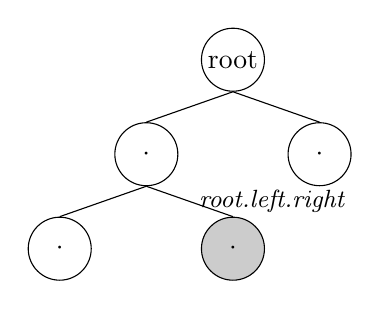
\begin{tikzpicture}[
  every node/.style={circle, draw, minimum size=8mm, inner sep=0pt},
  level distance=12mm, sibling distance=22mm
]
\node {root}
  child { node {$\cdot$}
    child { node {$\cdot$} }
    child { node[fill=black!20] {$\cdot$}
      edge from parent node[draw=none, right, xshift=3pt]{\small\textit{root.left.right}}
    }
  }
  child { node {$\cdot$} };
\end{tikzpicture}
\end{center}

Given only the root node of a heap represented as a recursive node structure of $n$ nodes, $n$, and a number $x$, give an efficient algorithm to insert $x$ into the heap and analyze its runtime. You don't need to redescribe how upheap works.

Hint: It's possible to do better than linear time.

\textbf{Key insight:} A heap is a complete binary tree. Nodes in level-order are numbered $1, 2, \ldots, n$ (root = 1), and the next insertion point is position $n+1$. Writing $n+1$ in binary as $1\,b_{m-1}\,b_{m-2}\,\ldots\,b_1\,b_0$, the path from the root to position $n+1$ is exactly the bits $b_{m-1}, \ldots, b_0$: take a \emph{left} child for a 0-bit and a \emph{right} child for a 1-bit. This lets us navigate directly to the insertion point in $O(\log n)$ time without a linear scan.

\textbf{High-level description:} Decode $n+1$ into its binary path bits. Traverse from the root following those bits (skipping the leading 1) to reach the parent of the insertion point. Attach the new node as the appropriate child, then run upheap to restore the heap property.

\begin{verbatim}
insert(root, n, x):
  newNode = new Node(x)
  if n == 0:
    return newNode

  target = n + 1
  bits = []
  temp = target
  while temp > 1:
    bits.append(temp % 2)
    temp = temp // 2
  reverse(bits)

  current = root
  for i from 0 to len(bits) - 2:
    if bits[i] == 0: current = current.left
    else:            current = current.right

  newNode.parent = current
  if bits[len(bits) - 1] == 0:
    current.left  = newNode
  else:
    current.right = newNode

  // Restore heap-order property
  upheap(newNode)

  return root
\end{verbatim}

\textbf{Correctness:} The binary encoding of level-order position $k$ uniquely specifies the root-to-node path (standard complete binary tree property). Inserting at position $n+1$ maintains the complete-tree invariant. Upheap then restores the heap-order property by swapping values up the tree until the heap property holds.

\textbf{Runtime:} The binary representation of $n+1$ has $\lfloor\log_2(n+1)\rfloor + 1$ bits, so path traversal takes $O(\log n)$. Upheap traverses at most the tree height, also $O(\log n)$. Total: $O(\log n)$.

%%%

\end{questions}

\end{document}
